\documentclass[twoside]{book}

% Packages required by doxygen
\usepackage{fixltx2e}
\usepackage{calc}
\usepackage{doxygen}
\usepackage[export]{adjustbox} % also loads graphicx
\usepackage{graphicx}
\usepackage[utf8]{inputenc}
\usepackage{makeidx}
\usepackage{multicol}
\usepackage{multirow}
\PassOptionsToPackage{warn}{textcomp}
\usepackage{textcomp}
\usepackage[nointegrals]{wasysym}
\usepackage[table]{xcolor}

% Font selection
\usepackage[T1]{fontenc}
\usepackage[scaled=.90]{helvet}
\usepackage{courier}
\usepackage{amssymb}
\usepackage{sectsty}
\renewcommand{\familydefault}{\sfdefault}
\allsectionsfont{%
  \fontseries{bc}\selectfont%
  \color{darkgray}%
}
\renewcommand{\DoxyLabelFont}{%
  \fontseries{bc}\selectfont%
  \color{darkgray}%
}
\newcommand{\+}{\discretionary{\mbox{\scriptsize$\hookleftarrow$}}{}{}}

% Page & text layout
\usepackage{geometry}
\geometry{%
  a4paper,%
  top=2.5cm,%
  bottom=2.5cm,%
  left=2.5cm,%
  right=2.5cm%
}
\tolerance=750
\hfuzz=15pt
\hbadness=750
\setlength{\emergencystretch}{15pt}
\setlength{\parindent}{0cm}
\setlength{\parskip}{3ex plus 2ex minus 2ex}
\makeatletter
\renewcommand{\paragraph}{%
  \@startsection{paragraph}{4}{0ex}{-1.0ex}{1.0ex}{%
    \normalfont\normalsize\bfseries\SS@parafont%
  }%
}
\renewcommand{\subparagraph}{%
  \@startsection{subparagraph}{5}{0ex}{-1.0ex}{1.0ex}{%
    \normalfont\normalsize\bfseries\SS@subparafont%
  }%
}
\makeatother

% Headers & footers
\usepackage{fancyhdr}
\pagestyle{fancyplain}
\fancyhead[LE]{\fancyplain{}{\bfseries\thepage}}
\fancyhead[CE]{\fancyplain{}{}}
\fancyhead[RE]{\fancyplain{}{\bfseries\leftmark}}
\fancyhead[LO]{\fancyplain{}{\bfseries\rightmark}}
\fancyhead[CO]{\fancyplain{}{}}
\fancyhead[RO]{\fancyplain{}{\bfseries\thepage}}
\fancyfoot[LE]{\fancyplain{}{}}
\fancyfoot[CE]{\fancyplain{}{}}
\fancyfoot[RE]{\fancyplain{}{\bfseries\scriptsize Generated by Doxygen }}
\fancyfoot[LO]{\fancyplain{}{\bfseries\scriptsize Generated by Doxygen }}
\fancyfoot[CO]{\fancyplain{}{}}
\fancyfoot[RO]{\fancyplain{}{}}
\renewcommand{\footrulewidth}{0.4pt}
\renewcommand{\chaptermark}[1]{%
  \markboth{#1}{}%
}
\renewcommand{\sectionmark}[1]{%
  \markright{\thesection\ #1}%
}

% Indices & bibliography
\usepackage{natbib}
\usepackage[titles]{tocloft}
\setcounter{tocdepth}{3}
\setcounter{secnumdepth}{5}
\makeindex

% Hyperlinks (required, but should be loaded last)
\usepackage{ifpdf}
\ifpdf
  \usepackage[pdftex,pagebackref=true]{hyperref}
\else
  \usepackage[ps2pdf,pagebackref=true]{hyperref}
\fi
\hypersetup{%
  colorlinks=true,%
  linkcolor=blue,%
  citecolor=blue,%
  unicode%
}

% Custom commands
\newcommand{\clearemptydoublepage}{%
  \newpage{\pagestyle{empty}\cleardoublepage}%
}

\usepackage{caption}
\captionsetup{labelsep=space,justification=centering,font={bf},singlelinecheck=off,skip=4pt,position=top}

%===== C O N T E N T S =====

\begin{document}

% Titlepage & ToC
\hypersetup{pageanchor=false,
             bookmarksnumbered=true,
             pdfencoding=unicode
            }
\pagenumbering{roman}
\begin{titlepage}
\vspace*{7cm}
\begin{center}%
{\Large My Project }\\
\vspace*{1cm}
{\large Generated by Doxygen 1.8.11}\\
\end{center}
\end{titlepage}
\clearemptydoublepage
\tableofcontents
\clearemptydoublepage
\pagenumbering{arabic}
\hypersetup{pageanchor=true}

%--- Begin generated contents ---
\chapter{Todo List}
\label{todo}
\hypertarget{todo}{}

\begin{DoxyRefList}
\item[\label{todo__todo000002}%
\hypertarget{todo__todo000002}{}%
Member \hyperlink{structg1_1_1packet_a885a0ecdce163a529a58cc9b53ff323b}{g1\+:\+:packet\+:\+:ackcounts} ]
\item[\label{todo__todo000001}%
\hypertarget{todo__todo000001}{}%
Member \hyperlink{structg1_1_1packet_a3a260b0ab8300cd034be8a023ff8189d}{g1\+:\+:packet\+:\+:last\+\_\+ack} ]
\end{DoxyRefList}
\chapter{Class Index}
\section{Class List}
Here are the classes, structs, unions and interfaces with brief descriptions\+:\begin{DoxyCompactList}
\item\contentsline{section}{\hyperlink{structg1_1_1package__block}{g1\+::package\+\_\+block} \\*Структура-\/описатель блока. Создается поверх пакета для упрощения работы с ним }{\pageref{structg1_1_1package__block}}{}
\item\contentsline{section}{\hyperlink{structg1_1_1package__header}{g1\+::package\+\_\+header} \\*Структура заголовок пакета }{\pageref{structg1_1_1package__header}}{}
\end{DoxyCompactList}

\chapter{File Index}
\section{File List}
Here is a list of all documented files with brief descriptions\+:\begin{DoxyCompactList}
\item\contentsline{section}{/home/mirmik/project/g1/g1/{\bfseries gateway.\+h} }{\pageref{gateway_8h}}{}
\item\contentsline{section}{/home/mirmik/project/g1/g1/{\bfseries indexes.\+h} }{\pageref{indexes_8h}}{}
\item\contentsline{section}{/home/mirmik/project/g1/g1/\hyperlink{packet_8h}{packet.\+h} \\*Всё, что касается работы с пакетом }{\pageref{packet_8h}}{}
\item\contentsline{section}{/home/mirmik/project/g1/g1/\hyperlink{tower_8h}{tower.\+h} \\*Tower file }{\pageref{tower_8h}}{}
\end{DoxyCompactList}

\chapter{Class Documentation}
\hypertarget{structg1_1_1gateway}{}\section{g1\+:\+:gateway Struct Reference}
\label{structg1_1_1gateway}\index{g1\+::gateway@{g1\+::gateway}}


{\ttfamily \#include $<$gateway.\+h$>$}

\subsection*{Public Member Functions}
\begin{DoxyCompactItemize}
\item 
virtual void \hyperlink{structg1_1_1gateway_a5748219660a573356ab0e52f715eebbf}{send} (\hyperlink{structg1_1_1packet}{packet} $\ast$pack)=0
\begin{DoxyCompactList}\small\item\em Отправить пакет в целевой мир, согласно адресу стадии. \end{DoxyCompactList}\item 
int \hyperlink{structg1_1_1gateway_a8554ef0120b9fbb279087eb1d8c205dd}{receive\+\_\+handler} (void $\ast$buf, size\+\_\+t sz)
\begin{DoxyCompactList}\small\item\em Обработка пакета, пришедшего из другого мира. \end{DoxyCompactList}\end{DoxyCompactItemize}
\subsection*{Public Attributes}
\begin{DoxyCompactItemize}
\item 
dlist\+\_\+head \hyperlink{structg1_1_1gateway_a9b30f9f8c97681eb9b8ce01594200916}{lnk}\hypertarget{structg1_1_1gateway_a9b30f9f8c97681eb9b8ce01594200916}{}\label{structg1_1_1gateway_a9b30f9f8c97681eb9b8ce01594200916}

\begin{DoxyCompactList}\small\item\em встроенное поле списка. \end{DoxyCompactList}\item 
uint16\+\_\+t \hyperlink{structg1_1_1gateway_a9bc58cdaebf54c916deb87c4c44c0a59}{id}\hypertarget{structg1_1_1gateway_a9bc58cdaebf54c916deb87c4c44c0a59}{}\label{structg1_1_1gateway_a9bc58cdaebf54c916deb87c4c44c0a59}

\begin{DoxyCompactList}\small\item\em номер врат. \end{DoxyCompactList}\item 
gxx\+::dlist$<$ \hyperlink{structg1_1_1packet}{packet},\&\hyperlink{structg1_1_1packet_ad385dbb95d429aa9616059bd374b359b}{packet\+::lnk} $>$ \hyperlink{structg1_1_1gateway_af6c41db1fccaf674f06a8c0893238c1d}{packq}\hypertarget{structg1_1_1gateway_af6c41db1fccaf674f06a8c0893238c1d}{}\label{structg1_1_1gateway_af6c41db1fccaf674f06a8c0893238c1d}

\begin{DoxyCompactList}\small\item\em Очередь пакетов, ожидающих отправки. \end{DoxyCompactList}\end{DoxyCompactItemize}


\subsection{Detailed Description}
Абстрактный класс врат. Врата отвечают за пересылку пакетов между мирами. 

\subsection{Member Function Documentation}
\index{g1\+::gateway@{g1\+::gateway}!receive\+\_\+handler@{receive\+\_\+handler}}
\index{receive\+\_\+handler@{receive\+\_\+handler}!g1\+::gateway@{g1\+::gateway}}
\subsubsection[{\texorpdfstring{receive\+\_\+handler(void $\ast$buf, size\+\_\+t sz)}{receive_handler(void *buf, size_t sz)}}]{\setlength{\rightskip}{0pt plus 5cm}int g1\+::gateway\+::receive\+\_\+handler (
\begin{DoxyParamCaption}
\item[{void $\ast$}]{buf, }
\item[{size\+\_\+t}]{sz}
\end{DoxyParamCaption}
)}\hypertarget{structg1_1_1gateway_a8554ef0120b9fbb279087eb1d8c205dd}{}\label{structg1_1_1gateway_a8554ef0120b9fbb279087eb1d8c205dd}


Обработка пакета, пришедшего из другого мира. 

Здесь происходит реверт адреса и переправка в башню. \index{g1\+::gateway@{g1\+::gateway}!send@{send}}
\index{send@{send}!g1\+::gateway@{g1\+::gateway}}
\subsubsection[{\texorpdfstring{send(packet $\ast$pack)=0}{send(packet *pack)=0}}]{\setlength{\rightskip}{0pt plus 5cm}virtual void g1\+::gateway\+::send (
\begin{DoxyParamCaption}
\item[{{\bf packet} $\ast$}]{pack}
\end{DoxyParamCaption}
)\hspace{0.3cm}{\ttfamily [pure virtual]}}\hypertarget{structg1_1_1gateway_a5748219660a573356ab0e52f715eebbf}{}\label{structg1_1_1gateway_a5748219660a573356ab0e52f715eebbf}


Отправить пакет в целевой мир, согласно адресу стадии. 

Убить зверя. 
\begin{DoxyParams}{Parameters}
{\em pack} & Пересылаемый пакет \\
\hline
\end{DoxyParams}
\begin{DoxyReturn}{Returns}
Статус ошибки. 
\end{DoxyReturn}


The documentation for this struct was generated from the following file\+:\begin{DoxyCompactItemize}
\item 
/home/mirmik/project/g1/g1/gateway.\+h\end{DoxyCompactItemize}

\hypertarget{structg1_1_1packet}{}\section{g1\+:\+:packet Struct Reference}
\label{structg1_1_1packet}\index{g1\+::packet@{g1\+::packet}}


Структура-\/описатель блока. Создается поверх пакета для упрощения работы с ним.  




{\ttfamily \#include $<$packet.\+h$>$}



Collaboration diagram for g1\+:\+:packet\+:
\nopagebreak
\begin{figure}[H]
\begin{center}
\leavevmode
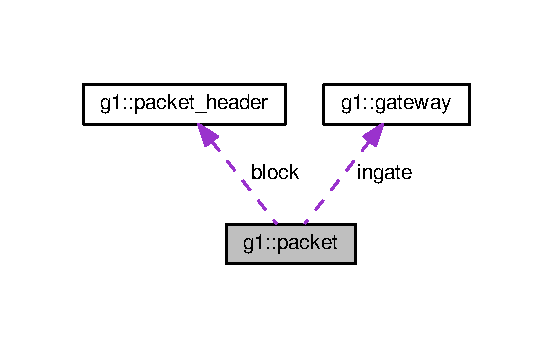
\includegraphics[width=266pt]{structg1_1_1packet__coll__graph}
\end{center}
\end{figure}
\subsection*{Public Member Functions}
\begin{DoxyCompactItemize}
\item 
void \hyperlink{structg1_1_1packet_ad49ed95720c1fa6cfaaa090cc656ba0e}{revert\+\_\+stage} (void $\ast$addr1, uint8\+\_\+t size1, void $\ast$addr2, uint8\+\_\+t size2, uint8\+\_\+t gateindex)\hypertarget{structg1_1_1packet_ad49ed95720c1fa6cfaaa090cc656ba0e}{}\label{structg1_1_1packet_ad49ed95720c1fa6cfaaa090cc656ba0e}

\begin{DoxyCompactList}\small\item\em Отметить в пакете прохождение врат. \end{DoxyCompactList}\item 
void {\bfseries revert\+\_\+stage} (void $\ast$addr, uint8\+\_\+t size, uint8\+\_\+t gateindex)\hypertarget{structg1_1_1packet_a1477ce6289dcf4f43fd8f13a1b67dcc2}{}\label{structg1_1_1packet_a1477ce6289dcf4f43fd8f13a1b67dcc2}

\item 
void {\bfseries revert\+\_\+stage} (uint8\+\_\+t gateindex)\hypertarget{structg1_1_1packet_aa874d40c216570159b4ca4e3a1ec9b3e}{}\label{structg1_1_1packet_aa874d40c216570159b4ca4e3a1ec9b3e}

\item 
uint8\+\_\+t {\bfseries gateway\+\_\+index} () const \hypertarget{structg1_1_1packet_a90a155e6bab5bcda6a30197fd9d5be35}{}\label{structg1_1_1packet_a90a155e6bab5bcda6a30197fd9d5be35}

\item 
gxx\+::buffer {\bfseries gateway\+\_\+address} (uint8\+\_\+t asz) const \hypertarget{structg1_1_1packet_a573fc5d020f3722647b960ff7ced4c4c}{}\label{structg1_1_1packet_a573fc5d020f3722647b960ff7ced4c4c}

\item 
bool {\bfseries is\+\_\+travelled} ()\hypertarget{structg1_1_1packet_a0de6bfa7627181490bd91164c33f38e1}{}\label{structg1_1_1packet_a0de6bfa7627181490bd91164c33f38e1}

\item 
char $\ast$ {\bfseries addrptr} ()\hypertarget{structg1_1_1packet_ada96086a5e461e198b226d8457470dcd}{}\label{structg1_1_1packet_ada96086a5e461e198b226d8457470dcd}

\item 
char $\ast$ {\bfseries dataptr} ()\hypertarget{structg1_1_1packet_afec6bda1de0b77ff21f34943daa5e04c}{}\label{structg1_1_1packet_afec6bda1de0b77ff21f34943daa5e04c}

\item 
char $\ast$ {\bfseries stageptr} ()\hypertarget{structg1_1_1packet_ad73d0cfaee06a9f92da17366b21e4532}{}\label{structg1_1_1packet_ad73d0cfaee06a9f92da17366b21e4532}

\item 
gxx\+::buffer {\bfseries addrsect} ()\hypertarget{structg1_1_1packet_ac3af772227e60f6bb522f54a19690461}{}\label{structg1_1_1packet_ac3af772227e60f6bb522f54a19690461}

\item 
gxx\+::buffer {\bfseries datasect} ()\hypertarget{structg1_1_1packet_a4fb1dd7f771981b0322ae6ef55b5400d}{}\label{structg1_1_1packet_a4fb1dd7f771981b0322ae6ef55b5400d}

\item 
void {\bfseries set\+\_\+type} (uint8\+\_\+t type)\hypertarget{structg1_1_1packet_a003cd27b118d0b74a40828224bc20504}{}\label{structg1_1_1packet_a003cd27b118d0b74a40828224bc20504}

\item 
void {\bfseries push\+\_\+addr} (uint8\+\_\+t addr)\hypertarget{structg1_1_1packet_a88b4e9d93ba038bfb13e465ec48c6a70}{}\label{structg1_1_1packet_a88b4e9d93ba038bfb13e465ec48c6a70}

\item 
void {\bfseries push\+\_\+addr} (gxx\+::buffer addr)\hypertarget{structg1_1_1packet_aa1e0166471e5a7cb52ac5f9dcec55530}{}\label{structg1_1_1packet_aa1e0166471e5a7cb52ac5f9dcec55530}

\item 
uint16\+\_\+t {\bfseries datasize} ()\hypertarget{structg1_1_1packet_afb750c10b51e0d1f5c337f6b0a142841}{}\label{structg1_1_1packet_afb750c10b51e0d1f5c337f6b0a142841}

\end{DoxyCompactItemize}
\subsection*{Public Attributes}
\begin{DoxyCompactItemize}
\item 
dlist\+\_\+head \hyperlink{structg1_1_1packet_ad385dbb95d429aa9616059bd374b359b}{lnk}\hypertarget{structg1_1_1packet_ad385dbb95d429aa9616059bd374b359b}{}\label{structg1_1_1packet_ad385dbb95d429aa9616059bd374b359b}

\begin{DoxyCompactList}\small\item\em Для подключения в список. \end{DoxyCompactList}\item 
\hyperlink{structg1_1_1gateway}{g1\+::gateway} $\ast$ \hyperlink{structg1_1_1packet_ae5b9f8200d6c128cd9a4a436c1f8d1dc}{ingate}\hypertarget{structg1_1_1packet_ae5b9f8200d6c128cd9a4a436c1f8d1dc}{}\label{structg1_1_1packet_ae5b9f8200d6c128cd9a4a436c1f8d1dc}

\begin{DoxyCompactList}\small\item\em gate, которым пакет прибыл в систему. \end{DoxyCompactList}\item 
uint16\+\_\+t \hyperlink{structg1_1_1packet_adeb6ae81faca9970d09c848a793d2a9f}{last\+\_\+request\+\_\+time}
\item 
uint8\+\_\+t \hyperlink{structg1_1_1packet_a18df7f0ed915a9b7901c73afce275f87}{ackcount}
\item 
\begin{tabbing}
xx\=xx\=xx\=xx\=xx\=xx\=xx\=xx\=xx\=\kill
union \{\\
\>uint8\_t \hyperlink{structg1_1_1packet_aeb31a298732861167f07f7ae38e25c07}{flags}\\
\>\>{\em Местные флаги }\\
\>struct \{\\
\>\>uint8\_t {\bfseries released\_by\_world}: 1\\
\>\>uint8\_t {\bfseries released\_by\_tower}: 1\\
\>\} \hypertarget{uniong1_1_1packet_1_1_0D4_a13673b76b09c9f880f62f539488b7117}{}\label{uniong1_1_1packet_1_1_0D4_a13673b76b09c9f880f62f539488b7117}
\\
\}; \hypertarget{structg1_1_1packet_af94d16abf234fdcfb447b00ed332ba9d}{}\label{structg1_1_1packet_af94d16abf234fdcfb447b00ed332ba9d}
\\

\end{tabbing}\item 
\hyperlink{structg1_1_1packet__header}{packet\+\_\+header} $\ast$ \hyperlink{structg1_1_1packet_a0647831e03bcc456f9d4349ac4db440e}{block}\hypertarget{structg1_1_1packet_a0647831e03bcc456f9d4349ac4db440e}{}\label{structg1_1_1packet_a0647831e03bcc456f9d4349ac4db440e}

\begin{DoxyCompactList}\small\item\em Указатель на заголовок реферируемого блока \end{DoxyCompactList}\end{DoxyCompactItemize}


\subsection{Detailed Description}
Структура-\/описатель блока. Создается поверх пакета для упрощения работы с ним. 

\subsection{Member Data Documentation}
\index{g1\+::packet@{g1\+::packet}!ackcount@{ackcount}}
\index{ackcount@{ackcount}!g1\+::packet@{g1\+::packet}}
\subsubsection[{\texorpdfstring{ackcount}{ackcount}}]{\setlength{\rightskip}{0pt plus 5cm}uint8\+\_\+t g1\+::packet\+::ackcount}\hypertarget{structg1_1_1packet_a18df7f0ed915a9b7901c73afce275f87}{}\label{structg1_1_1packet_a18df7f0ed915a9b7901c73afce275f87}
\begin{DoxyRefDesc}{Todo}
\item[\hyperlink{todo__todo000003}{Todo}]\end{DoxyRefDesc}
\index{g1\+::packet@{g1\+::packet}!last\+\_\+request\+\_\+time@{last\+\_\+request\+\_\+time}}
\index{last\+\_\+request\+\_\+time@{last\+\_\+request\+\_\+time}!g1\+::packet@{g1\+::packet}}
\subsubsection[{\texorpdfstring{last\+\_\+request\+\_\+time}{last_request_time}}]{\setlength{\rightskip}{0pt plus 5cm}uint16\+\_\+t g1\+::packet\+::last\+\_\+request\+\_\+time}\hypertarget{structg1_1_1packet_adeb6ae81faca9970d09c848a793d2a9f}{}\label{structg1_1_1packet_adeb6ae81faca9970d09c848a793d2a9f}
\begin{DoxyRefDesc}{Todo}
\item[\hyperlink{todo__todo000002}{Todo}]\end{DoxyRefDesc}


The documentation for this struct was generated from the following files\+:\begin{DoxyCompactItemize}
\item 
/home/mirmik/project/g1/g1/\hyperlink{packet_8h}{packet.\+h}\item 
/home/mirmik/project/g1/g1/src/\hyperlink{packet_8cpp}{packet.\+cpp}\end{DoxyCompactItemize}

\hypertarget{structg1_1_1packet__header}{}\section{g1\+:\+:packet\+\_\+header Struct Reference}
\label{structg1_1_1packet__header}\index{g1\+::packet\+\_\+header@{g1\+::packet\+\_\+header}}


Структура заголовок пакета.  




{\ttfamily \#include $<$packet.\+h$>$}

\subsection*{Public Attributes}
\begin{DoxyCompactItemize}
\item 
\begin{tabbing}
xx\=xx\=xx\=xx\=xx\=xx\=xx\=xx\=xx\=\kill
union \{\\
\>uint8\_t \hyperlink{structg1_1_1packet__header_a77b86061c82d26733d902eb73af5976c}{pflag}\\
\>\>{\em Флаги пакета }\\
\>struct \{\\
\>\>uint8\_t {\bfseries ack}: 1\\
\>\>uint8\_t {\bfseries vaddr}: 1\\
\>\>uint8\_t {\bfseries type}: 6\\
\>\} \hypertarget{uniong1_1_1packet__header_1_1_0D0_a4a3039864fea2668bb6bc713d929cd2a}{}\label{uniong1_1_1packet__header_1_1_0D0_a4a3039864fea2668bb6bc713d929cd2a}
\\
\}; \hypertarget{structg1_1_1packet__header_a51a68c60941af526631dac75cf46878f}{}\label{structg1_1_1packet__header_a51a68c60941af526631dac75cf46878f}
\\

\end{tabbing}\item 
uint16\+\_\+t \hyperlink{structg1_1_1packet__header_aed8789b03d7fa0c382855e97aaec4dd0}{flen}\hypertarget{structg1_1_1packet__header_aed8789b03d7fa0c382855e97aaec4dd0}{}\label{structg1_1_1packet__header_aed8789b03d7fa0c382855e97aaec4dd0}

\begin{DoxyCompactList}\small\item\em Полная длина пакета \end{DoxyCompactList}\item 
uint16\+\_\+t \hyperlink{structg1_1_1packet__header_a790712eb4ffb25fc506c895b183ca138}{seqid}\hypertarget{structg1_1_1packet__header_a790712eb4ffb25fc506c895b183ca138}{}\label{structg1_1_1packet__header_a790712eb4ffb25fc506c895b183ca138}

\begin{DoxyCompactList}\small\item\em Порядковый номер пакета. Присваивается отправителем. \end{DoxyCompactList}\item 
uint8\+\_\+t \hyperlink{structg1_1_1packet__header_aadecf162728b76d0c72b30c6fe90774f}{alen}\hypertarget{structg1_1_1packet__header_aadecf162728b76d0c72b30c6fe90774f}{}\label{structg1_1_1packet__header_aadecf162728b76d0c72b30c6fe90774f}

\begin{DoxyCompactList}\small\item\em Длина поля адреса. \end{DoxyCompactList}\item 
uint8\+\_\+t \hyperlink{structg1_1_1packet__header_a47c2109902b4ce5d558bbac33e0b626f}{stg}\hypertarget{structg1_1_1packet__header_a47c2109902b4ce5d558bbac33e0b626f}{}\label{structg1_1_1packet__header_a47c2109902b4ce5d558bbac33e0b626f}

\begin{DoxyCompactList}\small\item\em Поля стадии. Используется для того, чтобы цепочка врат знала, какую часть адреса обрабатывать. \end{DoxyCompactList}\item 
\hyperlink{packet_8h_a157fb77f1b8142697dc1b88efaae6a0a}{QoS} \hyperlink{structg1_1_1packet__header_a556522406f886708bb389d14375c79b4}{qos}\hypertarget{structg1_1_1packet__header_a556522406f886708bb389d14375c79b4}{}\label{structg1_1_1packet__header_a556522406f886708bb389d14375c79b4}

\begin{DoxyCompactList}\small\item\em Поле качества обслуживания. \end{DoxyCompactList}\end{DoxyCompactItemize}


\subsection{Detailed Description}
Структура заголовок пакета. 

Заголовок пакета располагается в первых байтах пакета. за заголовком следует поле адреса переменной длины, а за ним данные. 

The documentation for this struct was generated from the following file\+:\begin{DoxyCompactItemize}
\item 
/home/mirmik/project/g1/g1/\hyperlink{packet_8h}{packet.\+h}\end{DoxyCompactItemize}

\chapter{File Documentation}
\hypertarget{packet_8h}{}\section{/home/mirmik/project/g1/g1/packet.h File Reference}
\label{packet_8h}\index{/home/mirmik/project/g1/g1/packet.\+h@{/home/mirmik/project/g1/g1/packet.\+h}}


Всё, что касается работы с пакетом.  


{\ttfamily \#include $<$cstdint$>$}\\*
{\ttfamily \#include $<$gxx/buffer.\+h$>$}\\*
{\ttfamily \#include $<$gxx/datastruct/dlist\+\_\+head.\+h$>$}\\*
Include dependency graph for packet.\+h\+:
\nopagebreak
\begin{figure}[H]
\begin{center}
\leavevmode
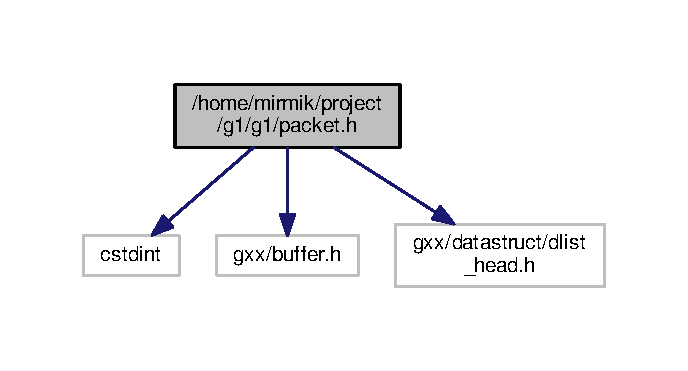
\includegraphics[width=330pt]{packet_8h__incl}
\end{center}
\end{figure}
This graph shows which files directly or indirectly include this file\+:
\nopagebreak
\begin{figure}[H]
\begin{center}
\leavevmode
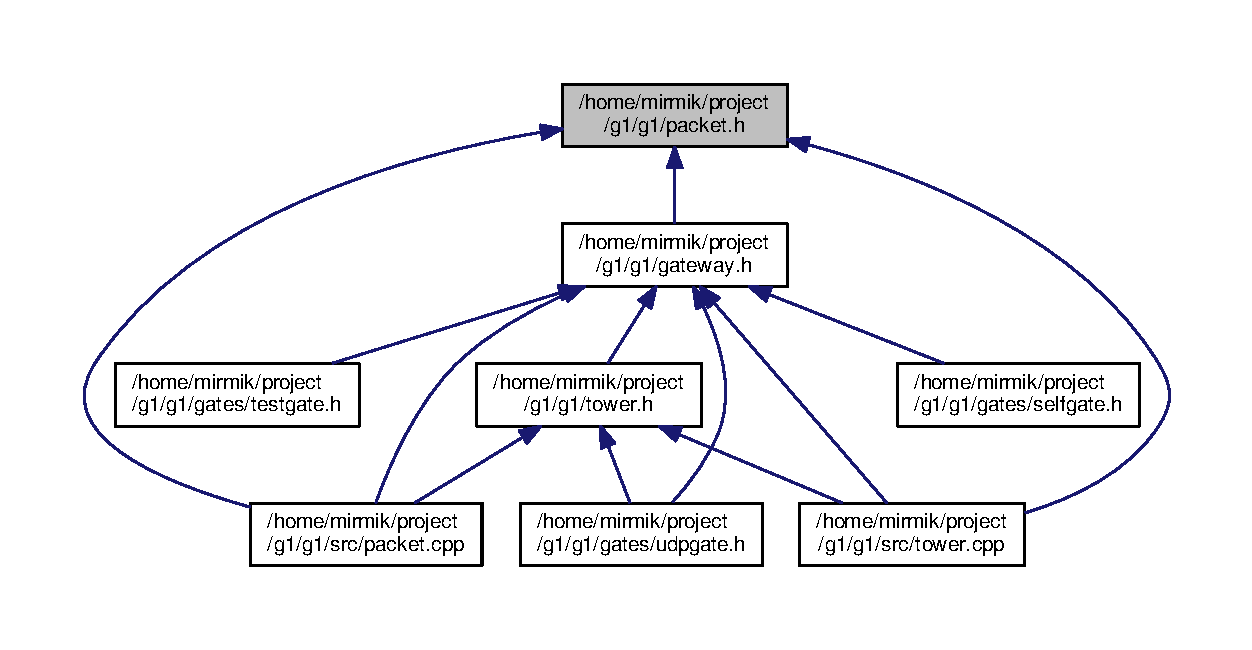
\includegraphics[width=188pt]{packet_8h__dep__incl}
\end{center}
\end{figure}
\subsection*{Classes}
\begin{DoxyCompactItemize}
\item 
struct \hyperlink{structg1_1_1packet__header}{g1\+::packet\+\_\+header}
\begin{DoxyCompactList}\small\item\em Структура заголовок пакета. \end{DoxyCompactList}\item 
struct \hyperlink{structg1_1_1packet}{g1\+::packet}
\begin{DoxyCompactList}\small\item\em Структура-\/описатель блока. Создается поверх пакета для упрощения работы с ним. \end{DoxyCompactList}\end{DoxyCompactItemize}
\subsection*{Macros}
\begin{DoxyCompactItemize}
\item 
\#define {\bfseries P\+A\+C\+K\+ED}~\+\_\+\+\_\+attribute\+\_\+\+\_\+((packed))\hypertarget{packet_8h_a36d525cf4d116b2fe4ecc00222b256f1}{}\label{packet_8h_a36d525cf4d116b2fe4ecc00222b256f1}

\end{DoxyCompactItemize}
\subsection*{Enumerations}
\begin{DoxyCompactItemize}
\item 
enum \hyperlink{packet_8h_a157fb77f1b8142697dc1b88efaae6a0a}{g1\+::\+QoS} \+: uint8\+\_\+t \{ \hyperlink{packet_8h_a157fb77f1b8142697dc1b88efaae6a0aafa5c8b0f0e32226b703768d3f4682a62}{g1\+::\+Without\+A\+CK} = 0, 
\hyperlink{packet_8h_a157fb77f1b8142697dc1b88efaae6a0aa4447997036a67abe0ac06f80015c7a55}{g1\+::\+Target\+A\+CK} = 1, 
\hyperlink{packet_8h_a157fb77f1b8142697dc1b88efaae6a0aa0c6f10580418c5118b9c4897a4e4a1c8}{g1\+::\+Binary\+A\+CK} = 2
 \}\begin{DoxyCompactList}\small\item\em Качество обслуживания. \end{DoxyCompactList}
\end{DoxyCompactItemize}
\subsection*{Functions}
\begin{DoxyCompactItemize}
\item 
packet\+\_\+header $\ast$ {\bfseries g1\+::allocate\+\_\+block} (uint8\+\_\+t asz, uint16\+\_\+t bsz)\hypertarget{packet_8h_a857314ea8a3d938fa526aa6f49411724}{}\label{packet_8h_a857314ea8a3d938fa526aa6f49411724}

\item 
packet\+\_\+header $\ast$ {\bfseries g1\+::create\+\_\+block} (uint8\+\_\+t asz, uint16\+\_\+t bsz)\hypertarget{packet_8h_ab68360f6a4657e000de452631a78d1c1}{}\label{packet_8h_ab68360f6a4657e000de452631a78d1c1}

\item 
void {\bfseries g1\+::utilize\+\_\+block} (packet\+\_\+header $\ast$block)\hypertarget{packet_8h_a27767df05aa0e656de62c4028f3ab147}{}\label{packet_8h_a27767df05aa0e656de62c4028f3ab147}

\item 
packet $\ast$ {\bfseries g1\+::allocate\+\_\+packet} ()\hypertarget{packet_8h_a28899956a502360c0535bc6e2231e2fb}{}\label{packet_8h_a28899956a502360c0535bc6e2231e2fb}

\item 
packet $\ast$ {\bfseries g1\+::create\+\_\+packet} (gateway $\ast$ingate, packet\+\_\+header $\ast$block)\hypertarget{packet_8h_a9efcb04e963d76617dc22ad8239c4fad}{}\label{packet_8h_a9efcb04e963d76617dc22ad8239c4fad}

\item 
void {\bfseries g1\+::utilize\+\_\+packet} (packet $\ast$pack)\hypertarget{packet_8h_a0a8be0f0a033b3a6a3921cb238472da6}{}\label{packet_8h_a0a8be0f0a033b3a6a3921cb238472da6}

\item 
void {\bfseries g1\+::utilize} (packet $\ast$pack)\hypertarget{packet_8h_a4538377a3f2665ec7b43a52a7813be10}{}\label{packet_8h_a4538377a3f2665ec7b43a52a7813be10}

\end{DoxyCompactItemize}
\subsection*{Variables}
\begin{DoxyCompactItemize}
\item 
struct \hyperlink{structg1_1_1packet__header}{g1\+::packet\+\_\+header} {\bfseries g1\+::\+P\+A\+C\+K\+ED}\hypertarget{packet_8h_ad5d8ed17112c281c66748354c4a54448}{}\label{packet_8h_ad5d8ed17112c281c66748354c4a54448}

\end{DoxyCompactItemize}


\subsection{Detailed Description}
Всё, что касается работы с пакетом. 



\subsection{Enumeration Type Documentation}
\index{packet.\+h@{packet.\+h}!QoS@{QoS}}
\index{QoS@{QoS}!packet.\+h@{packet.\+h}}
\subsubsection[{\texorpdfstring{QoS}{QoS}}]{\setlength{\rightskip}{0pt plus 5cm}enum {\bf g1\+::\+QoS} \+: uint8\+\_\+t}\hypertarget{packet_8h_file_a157fb77f1b8142697dc1b88efaae6a0a}{}\label{packet_8h_file_a157fb77f1b8142697dc1b88efaae6a0a}


Качество обслуживания. 

\begin{Desc}
\item[Enumerator]\par
\begin{description}
\index{Without\+A\+CK@{Without\+A\+CK}!packet.\+h@{packet.\+h}}\index{packet.\+h@{packet.\+h}!Without\+A\+CK@{Without\+A\+CK}}\item[{\em 
Without\+A\+CK\hypertarget{packet_8h_a157fb77f1b8142697dc1b88efaae6a0aafa5c8b0f0e32226b703768d3f4682a62}{}\label{packet_8h_a157fb77f1b8142697dc1b88efaae6a0aafa5c8b0f0e32226b703768d3f4682a62}
}]one \index{Target\+A\+CK@{Target\+A\+CK}!packet.\+h@{packet.\+h}}\index{packet.\+h@{packet.\+h}!Target\+A\+CK@{Target\+A\+CK}}\item[{\em 
Target\+A\+CK\hypertarget{packet_8h_a157fb77f1b8142697dc1b88efaae6a0aa4447997036a67abe0ac06f80015c7a55}{}\label{packet_8h_a157fb77f1b8142697dc1b88efaae6a0aa4447997036a67abe0ac06f80015c7a55}
}]two \index{Binary\+A\+CK@{Binary\+A\+CK}!packet.\+h@{packet.\+h}}\index{packet.\+h@{packet.\+h}!Binary\+A\+CK@{Binary\+A\+CK}}\item[{\em 
Binary\+A\+CK\hypertarget{packet_8h_a157fb77f1b8142697dc1b88efaae6a0aa0c6f10580418c5118b9c4897a4e4a1c8}{}\label{packet_8h_a157fb77f1b8142697dc1b88efaae6a0aa0c6f10580418c5118b9c4897a4e4a1c8}
}]three \end{description}
\end{Desc}

\hypertarget{tower_8h}{}\section{/home/mirmik/project/g1/g1/tower.h File Reference}
\label{tower_8h}\index{/home/mirmik/project/g1/g1/tower.\+h@{/home/mirmik/project/g1/g1/tower.\+h}}


tower file  


\subsection*{Functions}
\begin{DoxyCompactItemize}
\item 
void \hyperlink{tower_8h_a7fbcb90d84ad4b1dcdd2c09eac9c539c}{g1\+::transport} (\hyperlink{structg1_1_1package}{g1\+::package} pack)\hypertarget{tower_8h_a7fbcb90d84ad4b1dcdd2c09eac9c539c}{}\label{tower_8h_a7fbcb90d84ad4b1dcdd2c09eac9c539c}

\begin{DoxyCompactList}\small\item\em Переместить пакет дальше по конвееру врат. \end{DoxyCompactList}\item 
void \hyperlink{tower_8h_a750f6bfd94ccc8b6f47fc4fa94dd13bf}{g1\+::registry\+\_\+gate} (const \hyperlink{structg1_1_1gateway}{g1\+::gateway} \&gate)\hypertarget{tower_8h_a750f6bfd94ccc8b6f47fc4fa94dd13bf}{}\label{tower_8h_a750f6bfd94ccc8b6f47fc4fa94dd13bf}

\begin{DoxyCompactList}\small\item\em Подключить врата к башне. \end{DoxyCompactList}\end{DoxyCompactItemize}
\subsection*{Variables}
\begin{DoxyCompactItemize}
\item 
dlist$<$ \hyperlink{structg1_1_1gateway}{g1\+::gateway},\&\hyperlink{structg1_1_1gateway_a9b30f9f8c97681eb9b8ce01594200916}{g1\+::gateway\+::lnk} $>$ \hyperlink{tower_8h_a93a375fa1e7f88aa016b460f659ee244}{g1\+::gateways}\hypertarget{tower_8h_a93a375fa1e7f88aa016b460f659ee244}{}\label{tower_8h_a93a375fa1e7f88aa016b460f659ee244}

\begin{DoxyCompactList}\small\item\em Врата \end{DoxyCompactList}\end{DoxyCompactItemize}


\subsection{Detailed Description}
tower file 


%--- End generated contents ---

% Index
\backmatter
\newpage
\phantomsection
\clearemptydoublepage
\addcontentsline{toc}{chapter}{Index}
\printindex

\end{document}
